\chapter{单用户下的可验证对称加密搜索方案研究}
\label{cha:single-user}
\section{引言}
本章提出了一种普适的可验证对称加密搜索框架\single,该框架可以在单用户场景下工作,与任意对称加密搜索方案结合后,可以为用户提供加密搜索的结果验证服务。本章的主要内容安排如下:首先介绍了单用户场景下的系统框架,介绍了该框架的参与方及其所承担的计算任务;接着,通过一个正式定义从抽象层面介绍了该框架工作的流程和每个参与方涉及到的算法。随后,对\single 框架涉及到的算法进行了详细分析,包括数据持有者构建和更新验证索引的算法,云服务器搜索验证索引并生成结果证明的算法,数据持有者进行结果验证的算法。随后通过一个简单的例子对这几个算法进行了详细的阐述。最后,通过安全性分析和实验结果分析证明\single 方案可以达到设计目标中的安全性要求和性能要求。

\section{系统架构}
单用户场景下的可验证对称加密搜索框架如图~\ref{fig:GS-VSSE}所示,数据持有者即为数据搜索用户本身。初始化时需要数据持有者对自身的数据集进行加密,并对该数据集构建加密的验证索引,用于后续结果验证。数据持有者将加密文件集和验证索引上传给云服务器存储,并在需要时更新数据集和验证索引。当用户需要进行关键字搜索时,他将会构建出一个与关键字相关的搜索令牌,提交给云服务器进行搜索。云服务器接收到该搜索令牌后,通过某个加密搜索方案取得加密搜索结果,同时通过搜索验证索引取得一个结果证明,将加密搜索结果和结果证明返回给用户。用户在收到搜索结果和结果证明后,对其进行结果验证,若验证失败,则丢弃该结果。
\begin{figure}[t]
\centering
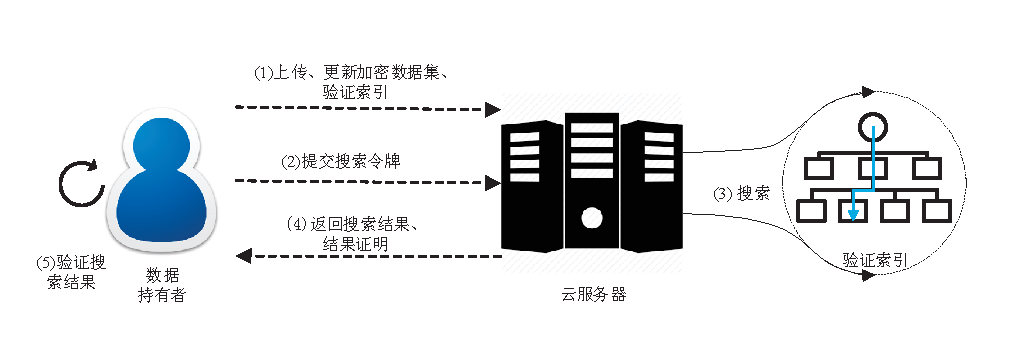
\includegraphics[width=6 in]{fig/GS-VSSE}
\DeclareGraphicsExtensions.
\caption{单用户场景下的可验证对称加密搜索框架\single}
\label{fig:GS-VSSE}
\end{figure}

\section{方案流程}

\begin{definition}[\textbf{\single 方案}]\label{def:single}
  {\itshape
      在\single 方案中,参与方有两个,分别为数据持有者本身和不可信的云服务器。数据持有者向云服务器提供加密数据集和验证索引,使得云服务器在用户搜索时可以向其返回结果证明,用于确保加密搜索结果的新鲜性和完整性。一个\single 方案是以下七个算法的集合:
      \begin{itemize}
        \item $KGen(1^k) \rightarrow \{K_1,K_2\}$: 是由数据持有者执行的秘钥生成算法。它将一个安全参数作为输入,输出对称秘钥$K_1,K_2$。
        \item $Init(K_1,K_2, \mathcal{D}) \rightarrow \{\lambda\}$: 是由数据持有者执行的初始化算法。它将对称秘钥$K_1,K_2$和明文文件集$\mathcal{D}$作为输入,输出验证索引$\lambda$。数据持有者在本地保存验证索引$\lambda$的根节点哈希$rt$,并将验证索引$\lambda$上传给云服务器。
        \item $UpdateToken(K_1,K_2, d) \rightarrow \{\tau_u\}$: 是由数据持有者执行的更新令牌生成算法。它将对称秘钥$K_1,K_2$和需要更新的文件$d$作为输入,输出一系列更新令牌$\tau_u$。数据持有者将更新令牌$\tau_u$上传给云服务器。
        \item $PreUpdate(\lambda, \tau_u) \rightarrow \{\lambda',\rho_u\}$: 是由云服务器执行的预更新算法。它将验证索引$\lambda$和更新令牌$\tau_u$作为输入,输出更新后的验证索引$\lambda'$,和更新证明$\rho_u$。云服务器将更新证明$\rho_u$返回给用户。
        \item $Update(rt,\tau_u,\rho_u) \rightarrow \{rt'\}$:是由数据持有者执行的更新算法。它将验证索引的根哈希 $rt$,更新令牌$\tau_u$和服务器返回的更新证明 $\rho_u$ 作为输入,输出新的根哈希$rt'$。若更新证明$\rho_u$验证通过,则输出更新后的根哈希$rt'$,若更新证明验证失败,则输出的根哈希$rt'$与原始根哈希$rt$相同。
        \item $SearchToken(K_1, w) \rightarrow \{\tau_{w}\}$: 是由数据持有者执行的搜索令牌生成算法。它将对称秘钥$K_1$和某一关键字$w$作为输入,输出与该关键字相关搜索令牌$\tau_{w}$。数据持有者将该搜索令牌 $\tau_{w}$上传给云服务器进行搜索。
        \item $Prove(\lambda, \tau_{w}) \rightarrow \{\rho_s\}$: 是由云服务器执行的搜索算法。它将验证索引$\lambda$和搜索令牌$\tau_{w}$作为输入,输出结果证明$\rho$。云服务器将结果证明$\rho$返回给数据持有者。
        \item $Verify(K_1,K_2, C_w, \tau_{w}, rt) \rightarrow \{b\}$: 是由数据持有者执行的验证算法。它将对称秘钥$K_1,K_2$,加密搜索结果$C_w$,搜索令牌$\tau_{w}$和保留的验证索引根哈希$rt$作为输入,输出一个比特$b$,代表接受或者拒绝该搜索结果。
      \end{itemize}
      }
\end{definition}
注意,上述流程中的每一个算法(除了$Verify$算法),都与加密搜索流程中的算法一一对应。例如$Init$,$UpdateToken$,$PreUpdate$算法可以与加密搜索中的初始化和更新操作同时进行,$Prove$算法可以与加密搜索中的搜索操作同时进行。该可验证加密搜索方案带来的额外算法是$Verify$算法,它用于用户收到搜索结果后的验证操作。正式因为\single 方案的每一个算法都从加密搜索方案中解耦了出来,才使得该方案可以将加密搜索方案当做黑盒,并为任意加密搜索方案提供结果验证服务。

\section{算法分析}
本节,我们将具体阐述\single 方案,即单用户场景下的可验证加密搜索框架。首先我们将描述如何建立并更新验证索引,然后我们将给出服务器生成结果证明的方法,并详细解释用户如何利用结果证明来确保搜索结果的正确性。

\subsection{构建及更新验证索引}
\begin{algorithm}[ht]
  \caption{$Init$ 算法}
  \label{alg:Init}
  \begin{algorithmic}[1]
    \REQUIRE ~~\\{$K_1,K_2$: 对称秘钥; $\mathcal{D}$: 明文文件集合;  $F, G: \{0, 1\}^k \times \{0, 1\}^* \rightarrow \{0, 1\}^*$ 伪随机函数; $IH: \{0, 1\}^* \rightarrow \{0, 1\}^k$ 增量哈希函数; $H: \{0, 1\}^* \rightarrow \{0, 1\}^k$ 哈希函数}
    \ENSURE ~~\\{$\lambda$: 通过MPT构建的验证索引。}
              \FOR {each $w_i \in \Delta$, 其中 $\Delta$ 是包括了$<w_i, D_{w_i}>$ 的倒排索引, $i \in \{1,\cdot, |W|\}$。}
                \STATE{加密关键字作为“键” $\tau_{w_i} = F_{K_1}(w_i)$。}
                \STATE{加密包含该关键字的文件集合作为“值” $V_{w_i} = \sum_{f_i \in D_{w_i}}IH (G_{K_2} (f_i))$。}
                \STATE{向MPT插入键值对 $\lambda = \lambda.Insert (\tau_{w_i},V_{w_i})$。}
              \ENDFOR
              \RETURN 返回从MPT构建得到的验证索引 $\lambda$。
  \end{algorithmic}
\end{algorithm}

算法~\ref{alg:Init} 给出了建立验证索引的伪代码。首先数据持有者根据明文文件集$\mathcal{D}$计算出倒排索引$\Delta$,其中倒排索引$\Delta$是指关键字$w_i$与包含该关键字的文件$D_{w_i}$组成的索引。对倒排索引中的每一个关键字$w_i$,我们计算他的"键值对",其中“键”是每一个关键字通过伪随机函数生成的令牌,而“值”是包含该关键字的文件的增量哈希和。我们通过将这些“键值对”插入MPT中来形成验证索引。

\begin{algorithm}[ht]
  \caption{$Update$ 算法}
  \label{alg:update}
  \begin{algorithmic}[1]
    \REQUIRE ~~\\{$rt$: 验证索引的根哈希; $\tau_u$:更新令牌;$\rho_u$: 更新证明;}
    \ENSURE ~~\\{$rt'$: 更新后的根哈希。}
              \STATE{将更新令牌$\tau_u$解析为键值对($\tau_{w_i}$,$G_{K_2}(d)$),其中$i \in \{1,\cdot,|W_d|\}$,$d$为待更新的文件。}
              \FOR {each $\tau_{w_i} \in \tau_u$}
                \STATE{计算$rt_t = Compute(\tau_{w_i}, \rho_u)$。}
                \IF{$rt_t != rt$}
                  \RETURN{验证失败,返回原有根哈希$rt$。}
                \ENDIF
              \ENDFOR
              \STATE{计算$rt' = Compute(\tau_u,\rho)$。}
              \RETURN{验证成功,返回更新后的根哈希 $rt'$。}
  \end{algorithmic}
\end{algorithm}

对验证索引的更新操作支持三种方式,即插入、删除和编辑文件,其中编辑文件相当于删除一个文件后再新增一个文件。对于插入新文件操作,我们首先解析该文件$d$,得到该文件包含的关键字集合$W_d$,对每一个关键字$w_i \in W_d$,我们都用伪随机函数生成他的令牌$\tau_(w_i )$,并将文件的伪随机结果$G_{K_2}(d)$同时上传给云。云服务器收到后通过更新令牌$\tau_(w_i )$找到对应的叶子节点,并将$IH(G_{K_2}(d))$与原有的叶子节点的值相加。删除操作同样,只是将原有的叶子节点的值减去$IH(G_{K_2}(d))$。云服务器在更新每一个令牌时,都需要将该令牌对应的搜索路径保存在更新证明$\rho_u$中,用于后续发回给用户进行更新验证。


算法\ref{alg:update}展示了数据持有者在收到云服务器返回的更新证明$\rho_u$后,执行的更新验证操作。由于数据持有者本身在本地并不保留验证索引$\lambda$,只保留验证索引的根哈希$rt$,因此在数据产生更新时,如何更新该根哈希$rt$十分重要。因为云服务器是不可信的,数据持有者在提交了更新令牌$\tau_u$后,无法确保服务器执行了正确的更新操作,因此他需要云服务器返回更新证明$\rho_u$来进行验证。服务器返回的更新证明$\rho_u$包含了更新令牌$\tau_u$中每一个关键字令牌对应在验证索引$\lambda$上的路径。用户在接受到该更新证明后,首先将自身生成的更新令牌$\tau_u$解析为($\tau_{w_i}$,$G_{K_2}(d)$),随后对每一个令牌$\tau_{w_i}$,验证是否根据更新证明$\rho_u$生成原始根哈希$rt$。若每个令牌都能验证成功,则用户通过更新令牌$\tau_u$和更新验证$\rho_u$构建新的根哈希$rt'$,否则验证失败,用户保留原有根哈希$rt$。
在本章第\ref{sec:example}节,我们将通过一个例子来说明建立和更新验证索引的过程。


\subsection{生成结果证明}
如算法\ref{alg:Prove}所示,服务器根据用户提交的搜索令牌$\tau_(w_i )$和验证索引$\lambda$来生成结果证明$\rho_s$。首先服务器根据搜索令牌$\tau_(w_i )$来寻找搜索路径$\sigma$。如果搜索令牌$\tau_(w_i )$对应的叶子节点存在,即用户查询的关键字存在,则服务器从叶子节点的上一层节点开始,返回搜索路径上的“键”作为结果证明。注意对于分支节点,服务器还需要返回不在搜索路径上的“键值对”。如果搜索令牌$\tau_(w_i)$对应的叶子节点不存在,即用户查询的关键字不存在,则服务器需要从搜索终结的节点开始向上返回搜索路径中的“键”作为结果证明,而对于搜索的终结节点,服务器需要返回完整的键值对。
我们将在本章第\ref{sec:example}节,通过一个具体的例子来说明该过程。

\begin{algorithm}[ht]
  \caption{$Prove$算法}
  \label{alg:Prove}
  \begin{algorithmic}[1]
    \REQUIRE {$\lambda$: 云服务器维护的验证索引; $\tau_{w_i}$: 用户提交的搜索令牌; }
    \ENSURE {$\rho_s$: 搜索结果的结果证明;}
              \STATE {查找搜索令牌$\tau_{w_i}$在验证索引$\lambda$上的对应路径 $\sigma =(n_0, \cdots, n_i, \cdots, n_m) \leftarrow \lambda.Search(\tau_{w_i})$, 其中 $n_i \in \{EN, BN, LN\}$, $n_0$ 为根节点。}
              \IF {$t_{w_i}$ 在验证索引中存在}
                \FOR {$i = m-1$ to $0$}
                  \IF {$n_i = BN$}
                    \STATE {$\rho_s = \rho_s \cup C_{n_i}$,其中 $C_{n_i}$ 包括分支节点中在搜索路径 $\sigma$ 上的"键"和不在搜索路径上的“键值对”。}
                  \ELSIF{$n_i = EN$}
                    \STATE {$\rho_s = \rho_s \cup C_{n_i}$,其中 $C_{n_i}$ 包括扩展节点中的“键”。}
                  \ELSE
                    \STATE{$\rho_s = \rho_s \cup C_{n_i}$,其中 $C_{n_i}$ 包括叶子节点中的“键值对”。}
                  \ENDIF
                \ENDFOR
              \ELSE %{$t_{w_i}$ not exits}
                \FOR {$i = m$ to $0$}
                    \STATE{Repeat steps 4-10}
                \ENDFOR
              \ENDIF
              \RETURN{$\rho_s$}
  \end{algorithmic}
\end{algorithm}

\subsection{结果验证}

\begin{algorithm}[t]
  \caption{Verify}
  \label{alg:verify}
  \begin{algorithmic}[1]
    \REQUIRE {$K_1,K_2$: 对称秘钥; $C_{w}$: 加密搜索结果; $\rho_s$: 加密搜索结果证明; $\tau_{w}$: 用户提交的搜索令牌;$rt$:用户本身保留的根哈希;}
    \ENSURE {$b \in \{0,1\}$, 如果 $b=1$, 表示结果验证成功,否则表示结果验证失败;}
          \STATE {计算剩余键 $\{remain\_key\}$ = String.match ($\tau_{w_i}$, keys in $\rho$)}
          \IF {$C_{w} = \emptyset$ \&\& $remain\_key = \emptyset$}
              \STATE {根据结果证明$\rho_s$自底向上计算根哈希$rt_t$;}
          \ELSIF {$C_{w} \neq \emptyset$ \&\& $remain\_key \neq \emptyset$}
              \STATE {计算 $\varphi = \sum_{f \in D_{w}}IH (G_{K_2} (f_i))$, 其中 $D_w$ 是 $C_w$ 对应的明文信息;}
              \STATE {计算叶子节点 $LN = Compute(\varphi, remain\_key)$}
              \STATE {根据结果证明 $\rho$ 和叶子节点$LN$ 自底向上计算根哈希$rt_t$.}
          \ELSE
              \RETURN {$0$}
          \ENDIF
          \IF{$rt = rt_t$}
            \RETURN{$1$}
          \ELSE
            \RETURN{$0$}
          \ENDIF
  \end{algorithmic}
\end{algorithm}

如算法~\ref{alg:verify} 所示,当用户收到了结果证明$\rho_s$时,就可以开始验证数据的新鲜性和完整性。首先用户通过搜索令牌$\tau_{w_i}$与结果证明$\rho_s$中的“键”进行匹配。如果结果证明$\rho_s$中的“键”是搜索令牌$\tau_{w_i}$的前缀,则$remain\_key$存储搜索令牌$\tau_{w_i}$与结果证明匹配完后剩余的键。如果结果证明$\rho_s$中的“键”不是搜索令牌$\tau_{w_i}$的前缀,那么$remain\_key$就置为$\emptyset$。如果搜索结果 $C_{w}$ 和 $remain\_key$ 都为空集,则我们通过结果证明$\rho_s$直接计算出根哈希值$rt_t$。如果二者都不为空,则我们首先通过搜索结果$C_{w}$和$remain\_key$生成叶子节点的哈希值,再通过结果证明$\rho_s$重建出根哈希值$rt_t$。除了这两种情况以外,我们就认为服务器故意返回了空结果或服务器篡改了结果证明的内容。最后,用户通过对比重建得到的根哈希$rt_t$和用户本身保留的根哈希$rt$是否相等来判断数据新鲜性和数据完整性。如果二者相等,则验证通过,如果二者不相等,则说明服务器少返回了搜索结果或者服务器篡改了结果证明。



\subsection{实例分析}
\label{sec:example}

\begin{figure}[ht]
\centering
\includegraphics[width=5 in]{fig/inverted-index}
\DeclareGraphicsExtensions.
\caption{一个简单的倒排索引}
\label{fig:inverted-index}
\end{figure}

\begin{figure}[ht]
\centering
\includegraphics[width=6 in]{fig/MPT}
\DeclareGraphicsExtensions.
\caption{由倒排索引和MPT构建的验证索引}
\label{fig:inverted-index}
\end{figure}


\begin{figure}[ht]
  \begin{minipage}[b]{0.49\textwidth}
    \includegraphics[width= 2.9 in]{fig/updateProof}
    \caption{更新证明}
    \label{fig:updateProof}
  \end{minipage}
  \begin{minipage}[b]{0.49\textwidth}
    \includegraphics[width= 3.2 in]{fig/resultProof}
    \caption{结果证明}
    \label{fig:resultProof}
  \end{minipage}
\centering
\end{figure}

如图4所示,我们将通过一个解释性的实例来说明建立和更新验证索引的过程,以及生成结果证明和通过结果证明重建根哈希的过程。
建立并更新验证索引:首先,我们假设数据拥有者有四个文件,分别为$f_1,f_2,f_3,f_4$,他们包含了四个关键字$w_1,w_2,w_3,w_4$,其对应关系如图4中的倒排索引所示。当包含关键字$w_2$和$w_5$的文件$f_5$新增时,对于已经存在的关键字$w_2$,我们只需将$IH(G_K(f_5))$添加到原有的叶子节点上。对于不存在的关键字$w_2$,我们需要创建一个新的叶子节点,并将$IH(G_K(f_5))$作为他的节点值。
生成并验证结果证明:(1)假设用户想要搜索的关键字为$w_2$,他提交的对应该关键字的挑战令牌为“a5432”。由于该关键字令牌在验证索引中已经存在,服务器可以找到与该令牌对应的搜索路径{BN1,EN1,BN2,LN3},根据Prove算法,服务器会返回除LN3以外的路径上的键值作为结果证明,如$C_n2,C_n1,C_n0$所示。用户在收到结果证明$C_n2,C_n1,C_n0$以后,可以根据该证明和搜索结构重新构建根哈希。首先用户将令牌“a5432”与结果证明中的键进行匹配,发现“a54”为令牌的前缀,remain\_key 为“32”,用户根据“32”以及搜索结果$f_2,f_5$重新生成节点LN3,并通过结果证明自底向上构建冲根哈希的值。最后用户通过比较重构得到的根哈希和在鉴别符中解密得到的根哈希,来判断数据是否完整,假如服务器只返回了文件$f_2$,那么重构得到的根哈希将与正确的根哈希不匹配。(2)假设用户搜索的关键字令牌为“a5433”,该令牌在验证索引中不存在,其搜索路径与“a5432”相同,不同的是,该令牌在LN3处发生了不匹配,服务器需要从LN3节点开始自底向上生成结果证明,如图4中的$C_n3,C_n2,C_n1,C_n0$所示。用户在收到该结果证明以后,由于发现令牌与结果证明中的键无法匹配,因此remain\_key被置空,用户将直接根据结果证明重构根哈希。同样,通过与正确的根哈希进行对比,如果不相同,则说明服务器篡改了结果证明,产生了恶意行为。


\section{安全性分析}
在本节,我们将对方案的安全性进行证明。方案的安全性主要分为两个部分,一个是机密性,另一个是可验证性。机密性是指敌手无法从验证索引和用户发送的令牌中获取文件和关键字的明文信息。可验证性是指当服务器返回不完整或者错误的结果时,用户不会验证通过。
首先,我们采用基于仿真的博弈(simulation-based game)来证明方案的机密性。
定义1(机密性) 考虑如下的概率性实验,假设A是一个有状态的敌手,S是有状态的仿真者,L是有状态的泄露函数:
真实实验($Real_A (k)$):一个挑战者采用$KGen(1^k)$生成了对称密钥K。敌手A选择了一个文件集D让挑战者通过${λ,π}←Initialization(K,D$)生成验证索引λ和鉴别符$π$并发回给A。同时敌手A生成了多项式数量级的查询q={w,f}。对每一个查询q,敌手A从从挑战者中获取到挑战令牌$τ_w$或者更新令牌$τ_u$。最后敌手A输出一个比特b。
理想实验($Ideal_(A,S) (k)$):敌手A选择一个文件集D。给定L(D),仿真者S生成并发送验证索引和鉴别符给A。敌手A生成了多项式数量级的查询q={w,f}。对每一个查询q,仿真者S返回给A恰当的令牌τ和鉴别符π。最后敌手A输出一个比特b。
如果对于任何多项式时间内的敌手A,都存在一个多项式时间内的仿真者S使得$$|Pr⁡[Real_A (k)=1]-Pr⁡[Ideal_(A,S) (k)=1] |≤negl(k)$$,那么我们就说方案是L-机密的。在具体证明之前,我们首先给出泄露函数L的定义:$L(D)=(|λ|,|π|,{τ}_q,{σ})$,其中$|λ|$表示验证索引的大小,以叶子节点的数目来衡量。$|π|$表示鉴别符的长度,${τ_q}$表示由q个查询产生的令牌,$\sigma$表示验证索引的搜索路径。我们有以下的定理:
定理1:如果F,G都是伪随机函数,那么方案就是L-机密的。
证明:首先,给定$L(D)=(|λ|,|π|,{τ}_q,{σ})$,S通过选择$|λ|$个随机键值对插入MPT中生成一个仿真的验证索引λ ̃,并且选择一个长度为|π|的随机字符串作为仿真鉴别符π ̃,由于在真实的验证索引中,键值对都是采用了伪随机函数F,G进行了伪随机化的,因此敌手将无法区分出真实的λ,π和仿真的λ ̃,π ̃。
模拟挑战令牌时,对于第一个挑战令牌$τ_w$,如果与{σ}中的某一路径匹配,那么S就在λ ̃中选择任意一条路径作为挑战令牌($τ_w $) ̃发送给敌手A,否则S就选择不在λ ̃路径中的随机字符串作为挑战令牌($τ_w $) ̃发送给敌手A。对于后续的挑战令牌,如果w之前出现过,那么挑战令牌($τ_w$ ) ̃就和之前发送给敌手的一样。如果w没出现过,那么挑战令牌的生成方式就和第一个令牌一样。由于令牌采用了伪随机函数F进行了加密,因此敌手A也无法区分真实的令牌和仿真的令牌。
模拟更新令牌时,更新令牌被设置为$(τ_u ) ̃=((τ_(w_1 ) ) ̃,⋯,(τ_(w_|W_f |  ) ) ̃,(τ_r ) ̃)$,鉴别符π ̃被设置为π长度相同的随机字符串。对每一个更新令牌$(τ_(w_i ) $) ̃,与模拟挑战令牌方法相同,由于每一个令牌都采用了伪随机函数F进行了加密,而且文件采用了伪随机函数G进行了加密,因此敌手A无法区分真实的令牌和文件与仿真的令牌和文件。因此我们可以得到结论:真实实验和仿真实验的输出结果是不可区分的。
定理2:如果哈希函数H和增量哈希函数IH是抗碰撞的,并且G是伪随机函数,那么方案就是可验证的。
证明:考虑服务器返回的搜索结果为 ($D_w $) ̃,正确的搜索结果为$D_w$,但是用户的Verify算法验证通过了($D_w$ ) ̃的情况。为了证明方案的可验证性,我们只需要证明Check算法和Rebuild算法的可验证性。首先,对于Check算法,由于鉴别符π是由数据拥有者解密的,而数据拥有者是可信的,因此鉴别符π的不可篡改性是由底层的对称加密技术所保证的。任何不具有对称密钥的第三方,不可能生成可以被用户验证通过的鉴别符。其次,对于Rebuild算法,存在两种可能验证通过,第一种是在计算($D_w $) ̃和$D_w$对应的伪随机值和增量哈希值时产生了碰撞,第二种是在生成根哈希的路径中产生了哈希碰撞。不管是哪一种,都可以推出哈希函数产生了碰撞或者伪随机函数产生了碰撞,但是哈希函数产生碰撞或者伪随机函数产生碰撞的可能性是小于一个可忽略的值的,因此,我们的方案是可验证的。

\section{实验结果}

\begin{figure}[bhpt]
\centering
  \begin{minipage}[b]{0.48 \textwidth}
    \includegraphics[width=\textwidth]{expr/initialization}
    \caption{$Init$ delays}
    \label{fig:init}
  \end{minipage}
  \begin{minipage}[b]{0.48 \textwidth}
    \includegraphics[width=\textwidth]{expr/update}
    \caption{$PreUpdate$ throughput}
    \label{fig:update}
  \end{minipage}

  \hspace{-40.0pt}
  \par \vspace{-10.pt}
  \hspace{-36.0pt}

  \begin{minipage}[b]{0.48 \textwidth}
    \includegraphics[width=\textwidth]{expr/proof}
    \caption{Proof cost of MPT}
    \label{fig:proof}
  \end{minipage}
  \begin{minipage}[b]{0.48 \textwidth}
    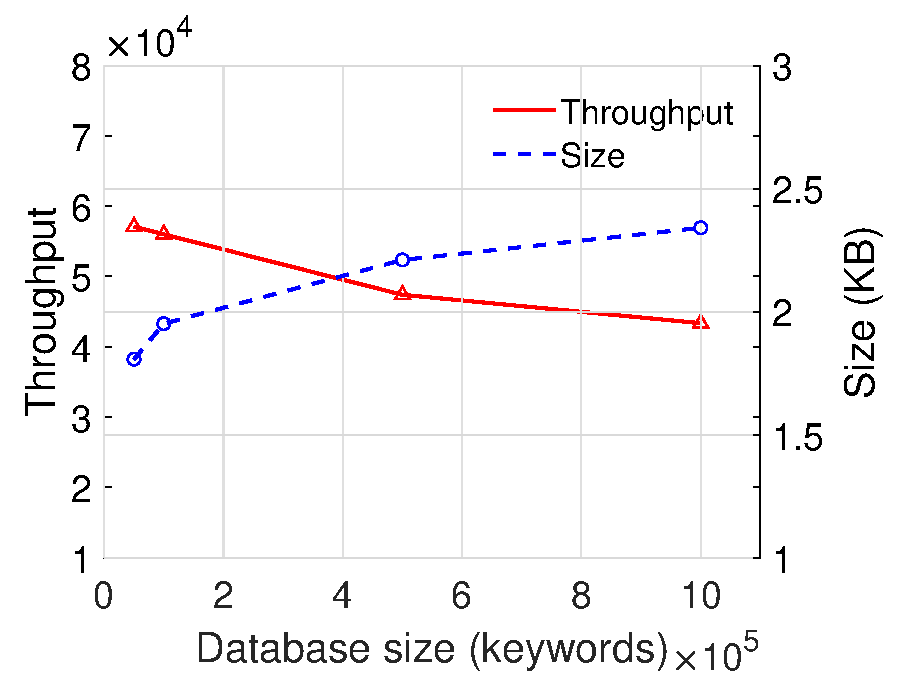
\includegraphics[width=\textwidth]{expr/prove}
    \caption{$Prove$ cost}
    \label{fig:prove}
  \end{minipage}

  \hspace{-40.0pt}
  \par \vspace{-10.pt}
  \hspace{-36.0pt}

  \begin{minipage}[b]{0.48 \textwidth}
    \includegraphics[width=\textwidth]{expr/verify}
    \caption{$Verify$ performance}
    \label{fig:verify}
  \end{minipage}
  \begin{minipage}[b]{0.48 \textwidth}
    \includegraphics[width=\textwidth]{expr/comparison}
    \caption{Comparison with SSE~\cite{cash2014dynamic}}
    \label{fig:comparison}
  \end{minipage}
\centering
\end{figure}

目前已经完成了实验测试和论文撰写。原型系统采用了Crypto5.6.5在C++上实现,包括测试代码在内总共2200多行代码。实验环境为Intel Core i5 2.5GHz处理器和4G内存,所有测试均采用单线程执行。实验采用了开源的Enron emails[17]作为测试数据,我们利用python脚本从其中提取出了关键字-文件对形成了倒排索引,注意提取关键字-文件对的时间不算在实验的测试时间范围内,因为该部分是和我们的方案独立的,取决于采用的文本提取算法。实验结果中给出的每一个数据点都是十次测试的平均值。

首先,如图5所示,生成验证索引的开销与文件-关键字对(document-keyword pair)的数目有关,因为有多少文件-关键字对,就需要执行多少次MPT的插入操作。从图中可以看出,当文件-关键字对的数目达到400万时,初始化生成验证索引的时间也只需要25秒左右,这对于初始化来说是可以接受的。
更新操作的延迟与MPT的大小有关,即与MPT中包含的关键字数目有关。关键字数目越多,MPT包含的叶子节点数目越多,MPT的大小就越大。严格上来说,更新的效率应该与MPT的层数有关,这里为了直观起见,我们采用关键字的数量来衡量MPT的大小,即数据库的大小。由于每个文件包含的关键字数目不等,因此我们采用吞吐量来衡量更新操作的效率,其中吞吐量代表了每秒钟可以执行多少个文件-关键字对的更新操作。从图6中可以看到,添加(Add)和删除(Delete)操作的吞吐量几乎相同。当数据库大小为100万时,每秒钟可以支持大约110000次更新操作。

如图7所示,当数据库大小为100万关键字时,服务器每秒钟可以执行大约43000次证明操作,这意味着服务器可以支持43000个用户的并发查询请求。而由结果证明带来的通信开销并不大,从图7中可以看出,每个结果证明的通信开销大约在2-3KB之间,结果证明的大小也与数据库的大小有关,但随着数据库的增长,结果证明的大小增长并不明显。
图8展示了用户对结果证明进行验证需要的时间,从图中可以看出,几乎100\%的验证可以在0.1毫秒内完成。


如图11所示,我们与动态加密搜索方案[3]进行了对比,我们采用了论文[3]中的实验结果作为基准,为了使得实验的对比更加公平,我们选择了相同的实验参数并且在最坏情况下进行了测量。通过提取16MB的邮件数据作为数据库大小,我们可以看到,我们的方案在搜索结果证明时,只需要18微秒的时间,而加密搜索的搜索时间由于与关键字包含的文件数量有关,因此平均搜索时间相对会比较大。对于添加和删除操作,加密搜索方案[3]在最坏情况下分别需要1.7微秒和113微秒时间,而我们的方案只需要0.7微秒。因此,可以说,我们的可验证加密搜索框架给加密搜索带来的额外开销并不大。


\begin{table}[h]
  \begin{center}
  \caption{Comparison with the SSE scheme proposed by Cash et al.~\cite{cash2014dynamic}}
  \label{tab:compareSSE}
  %\begin{threeparttable}
  \begin{tabular}{|c|c|c|}
    \hline
    Communication cost   & SSE~\cite{cash2014dynamic} &\single          \\
    \hline
    Search token          & 390 Bytes                 & 32 Bytes       \\
    \hline
    Search result/proof   & 53 Kilobytes              & 3 Kilobytes          \\
    \hline
  \end{tabular}
\end{center}
\end{table}
